\documentclass[10pt,a4paper]{article}
\usepackage[utf8]{inputenc}
\usepackage{amsmath}
\usepackage{amsfonts}
\usepackage{amssymb}
\usepackage{graphicx}
\usepackage{tikz}
\usetikzlibrary{automata,positioning}
\author{FILIP STENBECK	930702-4530 \\ ALEXANDER RAMM 931005-8418}
\date{Febuary 2016}
\title{Homework 2}
\begin{document}
\maketitle
\clearpage
\section*{Part 1:}
\subsection*{Rate Monotonic scheduling}
\subsubsection*{1}
Rate monotonic scheduling is a scheduling algorithm with fixed priorities. The highest priority is designated to the task with lowest period $T_i$. 
\subsubsection*{2}
The rate monotonic algorithm is schedulable if the Utilization factor ($U$) is less than $ln(2)$.
\begin{equation*}
U=\sum_{
   i=1
  }^{3}
 \frac{C_i}{T_i}<ln(2)
\end{equation*}
for these tasks with $C_1=C_2=C_3=6 ms$ the utilization factor is $0.6783$ which is less than $ln(2)$ thus schedulable.
\begin{figure}[!h]
  \centering
    \includegraphics[width=0.8\textwidth]{egen.jpg}
      \caption{The schedule for the three pendulums, for the first 70 ms.}
\end{figure}
\subsubsection*{3}
\begin{figure}[!ht]
  \centering
    \includegraphics[width=0.9\textwidth]{6ms.jpg}
      \caption{All three pendulums seems to be stable at execution time 6 ms.}
\end{figure}
The three pendulums have similar performances but we can see that there is no delay in the pendulum with highest priority (top plot) whilst the two other pendulums have a 6, 12 ms delay since they have lower priority. Due to that the system is schedulable we note that all the task are performed though with a maximum delay of 35 ms for the pendulum with lowest priority. 
\newpage
\subsubsection*{4}
\begin{figure}[!h]
  \centering
    \includegraphics[width=0.5\textwidth]{schedual6ms.jpg}
      \caption{The schedule for the three pendulums, highest priority is the bottom plot, lowest priority is the top plot. As we can see the analytic plot does seem to map to the schedule plot from simulink over the first 80 ms.}
\end{figure}
\subsubsection*{5}
For the tasks with $C_1=C_2=C_3=10 ms$ the utilization factor is $1.13$ which is higher than $ln(2)$ thus not schedulable. Note: Only the two tasks with the highest priority results in a utilization factor of $0.84$ which is still not schedulable, though this does not necessarily mean task 2 should be unstable as seen in figure \ref{1} but only that some data loss will happen.
\begin{figure}[!h]
  \centering
    \includegraphics[width=0.5\textwidth]{egen3.jpg}
      \caption{The schedule by hand, RM algorithm.}
\end{figure}
\begin{figure}[!h]
  \centering
    \includegraphics[width=0.5\textwidth]{schedual10ms.jpg}
      \caption{The schedule for the three pendulums execution time 10 ms. We can see that task 3 almost never get executed, though task 2 and 1 always get executed.}
\end{figure}
\begin{figure}[!h]\label{1}
  \centering
    \includegraphics[width=0.5\textwidth]{10ms.jpg}
      \caption{The pendulum with the lowest priority is now unstable at execution time 10 ms.}
\end{figure}
\newpage

\subsection*{Earliest deadline first}
\subsubsection*{1}
Earliest deadline first (EDF) is a dynamic scheduling algorithm. It calculates the closest deadline in absolute time and sets the priority according to that. This optimizes the computer time to the task in most need of it, thus making systems stable as long as the utilization factor is lower than 1. Since the algorithm is dynamic the computer need to continuously calculate the priorities of the tasks which does take some computation power and is slightly more complex than the predefined priorities from the rate monotonic algorithm.
\subsubsection*{2}  
The utilization factor is still $0.6783<1$ thus schedulable with this method.
\begin{figure}[!h]
  \centering
    \includegraphics[width=0.8\textwidth]{egen.jpg}
      \caption{The schedule for the three pendulums, for the first 70 ms. This is just the same as the rate monotonic algorithm for this interval.}
\end{figure}
\newpage
\subsubsection*{3}
Just like for the Rate monotonic algorithm for these execution times the three pendulums are stable. The shortest pendulum seem to have a little bit quicker response time. This is due to that it will be executed first at time $0(s)$. 
\begin{figure}[!ht]
  \centering
    \includegraphics[width=0.5\textwidth]{6msedf.jpg}
      \caption{All three pendulums seems to be stable at execution time 6 ms with the EDF algorithm.}
\end{figure}


\subsubsection*{4}
\begin{figure}[!ht]
  \centering
    \includegraphics[width=0.5\textwidth]{schedual6msedf.jpg}
      \caption{The schedule for the three pendulums,longest pendulum in the bottom plot, shortest in the top plot. As we can see the analytic plot maps to the schedule plot from simulink over the first 80 ms.}
\end{figure}
\newpage
\subsubsection*{5}
The utilization factor is still $1.13>1$ thus not schedulable with this method.
\begin{figure}[!h]
  \centering
    \includegraphics[width=0.8\textwidth]{egen2.jpg}
      \caption{The schedule for the three pendulums, for the first 70 ms. Execution time $C_i=10$ ms.}
\end{figure}
\begin{figure}[!h]
  \centering
    \includegraphics[width=0.5\textwidth]{schedual10msedf.jpg}
      \caption{The schedule for the three pendulums, at $C_i=10$ ms. We see that sometimes the first pendulum does not have the highest priority unlike the RM algorithm}
\end{figure}
\begin{figure}[!h]
  \centering
    \includegraphics[width=0.5\textwidth]{10msedf.jpg}
      \caption{The step response for the three pendulums with execution time 10 ms. We see that all three systems are stable unlike the RM algorithm, though we see that pendulum 1 has far worse performance.}
\end{figure}
\newpage
\subsubsection*{6}
in this case the control performances of all of the pendulums were stable for the EDF algorithm, whilst in the RM algorithm only two of the pendulums where stable for the long execution tie case. We would say that in this case the EDF is a better choice. Though keeping in mind that the different algorithms are just ways of distributing the brain power of the computer differently over the tasks. For example if the execution time would be even higher that the EDF algorithm would have none of the systems be stable might be a worse algorithm than having the RM algorithm stabilizing the one pendulum with highest priority.
\newpage
\newpage
\section*{Part 2:}
\subsection*{1. " Calculate analytically the closed-loop equations of the system."}
The following network control system is given. 
\begin{equation}
\dot{x}=Ax+Bu
\end{equation}\\ Where the matrices $A$, $B$ are set to be $0$, $I$ since the system is a simple integrator. The input $u$ is set to be. \\
\begin{equation*}
u=-Kx
\end{equation*}\\
In the network two delays are introduced. One before and one after the controller. This results in that the input of the system is delayed $\tau_{sc}+\tau_{ea}$ seconds. Since $\tau_{sc}+\tau_{ea}<h$ the input signal can be written.\\
\begin{equation}\label{knep1}
u=
\begin{cases}
u_0=-Kx(kh-h)&kh<t<kh+\tau_{sc}+\tau_{ea}\\
u_1=-Kx(kh)&kh+\tau_{sc}+\tau_{ea}<t<kh+h
\end{cases}
\end{equation}
With this we can formulate the closed loop equation.
\begin{equation*}
x(kh+h)=\mathrm{e}^{Ah}+\int_{kh}^{kh+h} \mathrm{e}^{AS}\,\mathrm{d}S Bu
\end{equation*}
\begin{equation}\label{knep2}
=\mathrm{e}^{Ah}x(kh)+\int_{kh}^{kh+\tau_{sc}+\tau_{ea}} \mathrm{e}^{AS}\,\mathrm{d}S Bu_0+\int_{kh+\tau_{sc}+\tau_{ea}}^{kh+h} \mathrm{e}^{AS}\,\mathrm{d}S Bu_1
\end{equation}
Setting the time delay $\tau=\tau_{sc}+\tau_{ea}$ and combining the equations \ref{knep1} with \ref{knep2} we result in the following closed loop equation.
\begin{equation*}
x(kh+h)=\begin{bmatrix}
1+K(\tau-h)&0\\
0&-K\tau
\end{bmatrix}
\begin{bmatrix}
x(kh)\\
x(kh-1)
\end{bmatrix}
\end{equation*}
\subsection*{2}
Since the continuous plant is a simple integrator $G(s)=\frac{1}{s}$ we get that the zero-order hold of the continuous plant will have the following pulse-transfer function.
\begin{equation*}
G(z)=\frac{h}{z-1}
\end{equation*}
With the controller as $C(z)=-K$ we will have a stable system if.
\begin{equation*}
|\frac{G(z)C(z)}{1+G(z)C(z)}|<\frac{1}{\tau z},	z\in R
\end{equation*}
This can be written as.
\begin{equation*}
hK(1-z\tau)<z-1,	z\in R
\end{equation*}
\subsection*{3}
The system becomes unstable approximately at $\tau=0.0398775$. This can we see through the output of the system that is plotted in figure \ref{2}below.
\begin{figure}[!h]\label{2}
  \centering
    \includegraphics[width=0.8\textwidth]{stable.jpg}
      \caption{The system becomes unstable approximately at $\tau=0.0398775$. Length of simulation 200 seconds. (Signal in black on white background.)}
\end{figure}
\section*{Task 3:}
\subsubsection*{1}
the machine $M_1$ and $M_2$ have the same statechart model in fig below.
\begin{center}

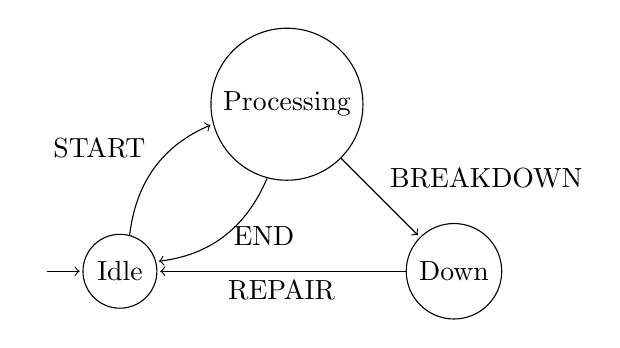
\begin{tikzpicture}[initial text=,shorten >=1pt,node distance=3cm,on grid,auto] 
   \node[state,initial] (q_0)   {Idle}; 
   \node[state] (q_1) [above right=of q_0] {Processing}; 
   \node[state](q_2) [below right=of q_1] {Down};
    \path[->] 
    (q_0) edge  [bend left] node {START} (q_1)
    (q_1) edge  node {BREAKDOWN} (q_2)
    		  edge [bend left, right] node {END } (q_0)
	(q_2) edge node {REPAIR} (q_0);
\end{tikzpicture}

\end{center}

The buffer has only two states:
\begin{center}
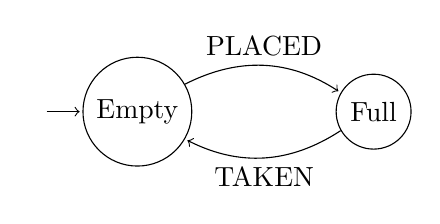
\begin{tikzpicture}[initial text=,shorten >=1pt,node distance=3cm,on grid,auto] 
   \node[state,initial] (q_0)   {Empty}; 
   \node[state] (q_1) [right=of q_0] {Full}; 
    \path[->] 
    (q_0) edge  [bend left, above] node {PLACED} (q_1)
    (q_1) edge [bend left, below] node {TAKEN} (q_0);
\end{tikzpicture}
\end{center}
\subsubsection*{2}
The state chart for the entire system can be seen below. It consists of all 18 possible states. Edges are not plotted due to space limitations.
\begin{center}
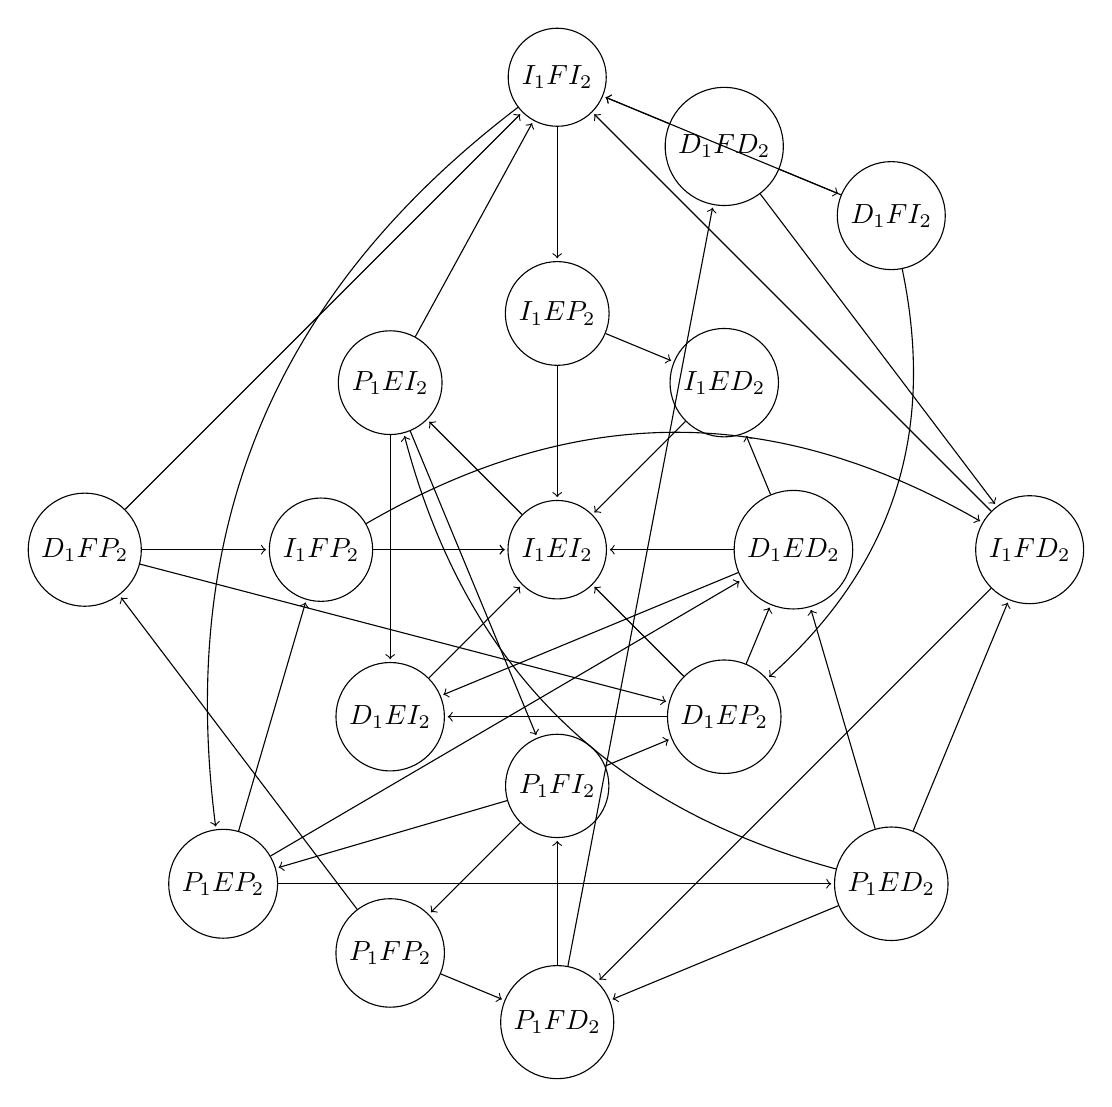
\begin{tikzpicture}[initial text=,shorten >=1pt,node distance=3cm,on grid,auto] 
   \node[state,initial] (IEI)   {$I_1EI_2$}; 
   \node[state] (IED) [above right=of IEI] {$I_1ED_2$}; 
   \node[state] (IEP) [above =of IEI]{$I_1EP_2$};
   \node[state] (PEI)   [above left=of IEI]{$P_1EI_2$}; 
   \node[state] (IFP) [left =of IEI]{$I_1FP_2$}; 
   \node[state] (DEI) [below left =of IEI]{$D_1EI_2$};
   \node[state] (DEP)   [below right=of IEI]{$D_1EP_2$}; 
   \node[state] (DED) [right =of IEI]{$D_1ED_2$}; 
   \node[state] (IFI) [above =of IEP]{$I_1FI_2$};
   \node[state] (PFI)   [below =of IEI]{$P_1FI_2$}; 
   \node[state] (DFD) [above right=of IEP]{$D_1FD_2$}; 
   \node[state] (DFI) [above right=of IED]{$D_1FI_2$};
   \node[state] (IFD)   [right =of DED]{$I_1FD_2$}; 
   \node[state] (DFP) [left=of IFP]{$D_1FP_2$}; 
   \node[state] (PFD) [below =of PFI]{$P_1FD_2$};
   \node[state] (PEP)  [below left =of DEI]{$P_1EP_2$}; 
   \node[state] (PED) [below right =of DEP]{$P_1ED_2$}; 
   \node[state] (PFP) [below left =of PFI]{$P_1FP_2$};
    \path[->] 
    (IEI) edge node {} (PEI)
    (IED) edge node {} (IEI)
    (IEP) edge node {} (IEI)
    		  edge node {} (IED)
    (PEI) edge node {} (PFI)
    	 	  edge node {} (DEI)
    	 	  edge node {} (IFI)
    (IFP) edge node {} (IEI)
    	      edge [bend left] node {} (IFD)
    (DEI) edge node {} (IEI)
    (DEP) edge node {} (IEI)
          edge node {} (DEI)
          edge node {} (DED)
    (DED) edge node {} (IEI)
          edge node {} (IED)
          edge node {} (DEI)
    (IFI) edge node {} (IEP)
    	      edge [bend right] node {} (PEP)
    (PFI) edge node {} (DEP)
          edge node {} (PFP)
          edge node {} (PEP)
    (DFD) edge node {} (DFI)
          edge node {} (IFD)
          edge node {} (IFI)
    (DFI) edge [bend left]node {} (DEP)
          edge node {} (IFI)
    (IFD) edge node {} (PFD)
          edge node {} (IFI)
    (DFP) edge node {} (IFI)
          edge node {} (DEP)
          edge node {} (IFP)
    (PFD) edge node {} (DFD)
          edge node {} (PFI) 
    (PEP) edge node {} (DED)
          edge node {} (PED)
          edge node {} (IFP)
    (PED) edge node {} (DED)
          edge [bend left]node {} (PEI)
          edge node {} (PFD)
          edge node {} (IFD)
    (PFP) edge node {} (DFP)
          edge node {} (PFD);
\end{tikzpicture}
\end{center}
\subsubsection*{3}
When applying the new rules some states becomes unreachable, and thus the model becomes simpler. All PF* states are no longer allowed and therefore DF* states can never be reached. Also some transitions have been removes to comply with the new rule set (DED$->$ IED for example), further simplifying the system. The new DES can be seen below:
\begin{center}
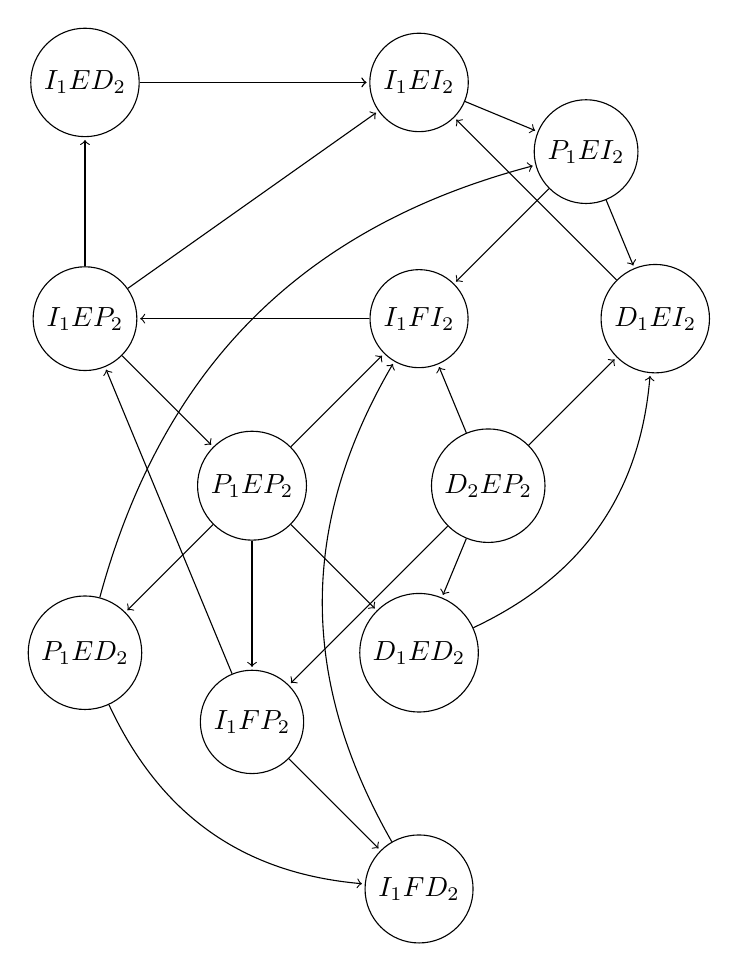
\begin{tikzpicture}[initial text=,shorten >=1pt,node distance=3cm,on grid,auto] 
   \node[state] (PEP)   {$P_1EP_2$}; 
   \node[state] (IFP) [below=of PEP] {$I_1FP_2$}; 
   \node[state] (PED) [below left =of PEP]{$P_1ED_2$};
   \node[state] (DED) [below right=of PEP]{$D_1ED_2$}; 
   \node[state] (IFI) [above right=of PEP]{$I_1FI_2$}; 
   \node[state] (IEP) [above left=of PEP]{$I_1EP_2$};
   \node[state] (IFD) [below right=of IFP]{$I_1FD_2$}; 
   \node[state] (DEI) [right =of IFI]{$D_1EI_2$}; 
   \node[state] (PEI) [above right =of IFI]{$P_1EI_2$};
   \node[state, initial] (IEI) [above =of IFI]{$I_1EI_2$}; 
   \node[state] (IED) [above =of IEP]{$I_1ED_2$};
   \node[state] (DEP) [right =of PEP]{$D_2EP_2$}; 
    \path[->] 
    (IEI) edge node {} (PEI)
    (IED) edge node {} (IEI)
    (IEP) edge node {} (IEI)
    		  edge node {} (IED)
    		  edge node {} (PEP)
    (PEI) edge node {} (DEI)
    	 	  edge node {} (IFI)
    (IFP) edge node {} (IEP)
    	      edge node {} (IFD)
    (PEP) edge node {} (IFI)
          edge node {} (PED)
          edge node {} (IFP)
          edge node {} (DED)
    (DEI) edge node {} (IEI)
    (DED) edge [bend right] node {} (DEI)
    (IFI) edge node {} (IEP)
    (IFD) edge [bend left] node {} (IFI)
    (PED) edge [bend left] node {} (PEI)
          edge [bend right] node {} (IFD)
    (DEP) edge node {} (DED)
    	      edge node {} (DEI)
    	      edge node {} (IFP)
    	      edge node {} (IFI);

\end{tikzpicture}
\end{center}
\subsubsection*{4}
If controlling $M_1$ and $M_2$ separately both controllers needs to be aware of the entire system state to be able to reach the allowed states and only the allowed states. If $M_1$ is down the controller need to know that $M_2$ is not down, therefore the two controllers must communicate with each other.

\end{document}